\chapter{Teorema di Reciprocità}
In un mezzo \textbf{lineare} e \textbf{isotropo}, i campi dovuti a sorgenti diverse sono legati dalla relazione:
\begin{squared}[violet]
    \int_{V_s} \bar{J}_1 \cdot \bar{E}_2 - \bar{J}_2 \cdot \bar{E}_1 dV + \int_{V_s} \bar{J}_{m2} \cdot \bar{H}_1 - \bar{J}_{m1} \cdot \bar{H}_2 dV = 0
\end{squared}
Applichiamo il \textbf{teorema} a un dispositivo con una porta in posizione $\bar{r}_1$ e l'altra in posizione $\bar{r}_2$:
\begin{center}
    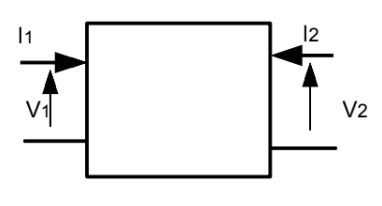
\includegraphics[width=.6\textwidth]{Images/figure35.png}
\end{center}
Dividiamo ora \textbf{due situazioni}:
\begin{center}
    \textbf{(a)}
\end{center}
\begin{center}
    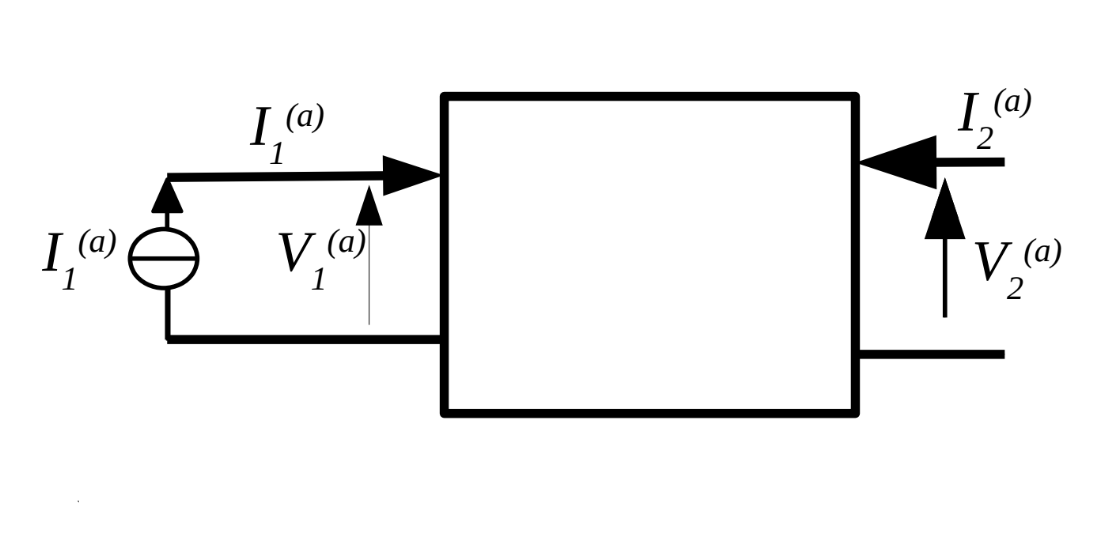
\includegraphics[width=.6\textwidth]{Images/figure36.png}
\end{center}
\begin{equation*}
    \bar{J}_1 = I_1^a \Delta \delta(|\bar{r} - \bar{r}_1|) \hat{i}_1
\end{equation*}
che produce:
\begin{equation*}
    \bar{E}_1 \quad e \quad \bar{H}_1
\end{equation*}

\begin{center}
    \textbf{(b)}
\end{center}
\begin{center}
    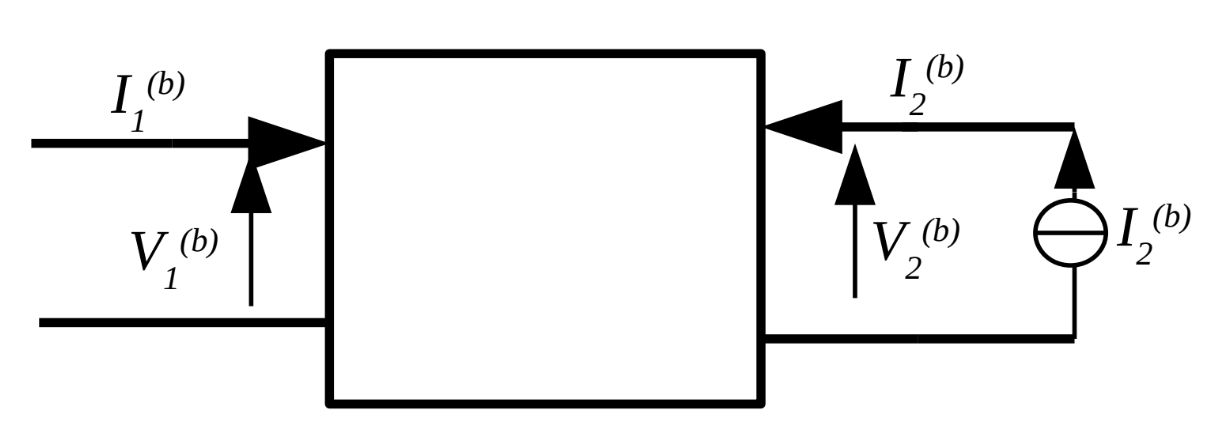
\includegraphics[width=.6\textwidth]{Images/figure37.png}
\end{center}
\begin{equation*}
    \bar{J}_2 = I_2^b \Delta \delta(|\bar{r} - \bar{r}_2|) \hat{i}_2
\end{equation*}
che produce:
\begin{equation*}
    \bar{E}_2 \quad e \quad \bar{H}_2
\end{equation*}
Sostituiamo nella \textbf{tesi}
\begin{equation*}
    \int_{V_s} I_1^a \Delta \delta(|\bar{r} - \bar{r}_1|) \hat{i}_1 \cdot \bar{E}_2 -  I_2^b \Delta \delta(|\bar{r} - \bar{r}_2|) \hat{i}_2 dV = 0
\end{equation*}
Ovvero:
\begin{equation*}
     I_1^a\Delta \int_{V_s}  \delta(|\bar{r} - \bar{r}_1|) \hat{i}_1 \cdot \bar{E}_2 dV =  I_2^b \Delta \int_{V_s}  \delta(|\bar{r} - \bar{r}_2|) \hat{i}_2 dV = 0
\end{equation*}
Che sfruttando la \textbf{proprietà della delta di Dirac} diventa:
\begin{equation*}
\tag{x}
     I_1^a\Delta\hat{i}_1 \bar{E}_2(\bar{r}_1) = I_2^b\Delta\hat{i}_2 \bar{E}_1(\bar{r}_2)
\end{equation*}
Possiamo assumere $\Delta$ \textbf{piccola} rispetto a $\lambda$, quindi possiamo considerare i \textbf{campi costanti} lungo $\Delta$, quindi:
\begin{equation*}
    V_1^b = - \int_{l_1} \bar{E}_2\cdot \hat{i}_1 dl = - \bar{E}_2(\bar{r}_1) \cdot \hat{i}_1 \Delta
\end{equation*}
che rappresenta la tensione alla porta 1 dovuta alla corrente $I_2^b$ alla porta 2.\\ \\
Analogamente:
\begin{equation*}
    V_2^a = - \int_{l_2} \bar{E}_1\cdot \hat{i}_2 dl = - \bar{E}_1(\bar{r}_2) \cdot \hat{i}_2 \Delta
\end{equation*}
Sostituendo in (x) otteniamo:
\begin{squared}
    I_1^a V_1^b = I_2^b V_2^a
\end{squared}











